%% -*- coding:utf-8 -*-
\frame[shrink=10]{
\frametitle{Argumente}

\begin{itemize}
\item Konstituenten stehen in verschiedenartigen Beziehungen zu ihrem Kopf.
\pause
\item Man unterscheidet zwischen \alert{Argumenten} und \alert{Adjunkten}.
\pause
\item Bestimmte Mitspieler (Aktanten) gehören zur Bedeutung eines Verbs.

\ZB gibt es in Situationen, die durch \emph{lieben} beschrieben werden,\\
immer einen \emph{Liebenden} und einen \emph{Geliebten} / etwas \emph{Geliebtes}.

\eal
\ex Conny liebt Aicke.
\ex $lieben'(Conny', Aicke')$
\zl

(\mex{0}b) ist eine logische Repräsentation für (\mex{0}a).

\relation{Conny} und \relation{Aicke} sind \alert{logische Argumente} von \relation{lieben}.

\pause
\item Syntaktische Argumente entsprechen meistens den logischen (später mehr).
\pause
\item Solche Beziehungen zwischen Kopf und Argumenten werden mit dem Begriff
\alert{Selektion} bzw.\ \alert{Valenz} erfasst.
\pause
\item \citet{Tesniere59a-u} überträgt Valenzbegriff aus der Chemie auf die Linguistik.
\end{itemize}

}


%\BackgroundPicture{periodensystem}{1}{1}
\frame{
\frametitle{Valenz in der Chemie}

\begin{itemize}
\item Atome können sich mit anderen Atomen zu mehr oder weniger stabilen Molekülen verbinden. 

\pause
\item Wichtig für die Stabilität ist, wie Elektronenschalen besetzt sind. 

\pause
\item Eine Verbindung mit anderen Atomen kann dazu führen,\\
dass eine Elektronenschale voll besetzt ist,\\
was dann zu einer stabilen Verbindung führt.

\pause
\item Die Valenz sagt etwas über die Anzahl der Wasserstoffatome aus,\\
die mit einem Atom eines Elements verbunden werden können. 

\pause
\item Sauerstoff hat die Valenz 2 und kann sich zu H$_2$O verbinden.

\pause
\item Man kann nun die Elemente in Valenzklassen einteilen.\\
Elemente mit einer bestimmten Valenz werden im Periodensystem von Mendeleev
in einer Spalte repräsentiert.

\end{itemize}

}

\frame{
\frametitle{Valenz in der Linguistik}

\begin{itemize}
\item Ein Kopf braucht bestimmte Argumente,\\
      um eine stabile Verbindung einzugehen. 

\pause
\item Kopf legt Form der Argumente fest (Kasus, Wortart).

\pause
\item Wörter mit der gleichen Valenz (mit gleicher Anzahl und Art von Argumenten)  werden in Valenzklassen eingeordnet, da sie sich in bezug
auf die Verbindungen, die sie eingehen, gleich verhalten. 


\bigskip

\centerline{
\begin{forest}
[O
  [H] 
  [H] ]
\end{forest}
\hspace{5em}
\begin{forest}
[lieben
 [Conny]
 [Aicke] ]
\end{forest}
}

\bigskip

Verbindung von Sauerstoff mit Wasserstoff und Verbindung
eines Verbs mit seinen Argumenten

\end{itemize}

\vfill

}

\frame{
\frametitle{Kopf legt Form der Argumente fest}

\eal
\ex Er unterstützt \gruen{ihn}. \hfill(NP und Kasus der NP)
\ex Er hilft \gruen{ihm}. \hfill(NP und Kasus der NP)
\ex Er wartet \gruen{auf ihn}. \hfill(PP, Form der P  und Kasus der NP innerhalb)
\zl



}

\frame{
\frametitle{Optionale Argumente}

\begin{itemize}
\item Argumente müssen nicht immer realisiert werden:
\eal
\ex Er wartet auf den Installateur.
\ex Er wartet.
\zl
\pause
Das Präpositionalobjekt von \emph{warten} 
ist ein \alert{fakultatives Argument}.

\pause
\item In nominalen Umgebungen sind Argumente immer optional!
\eal
\ex Jemand liest diese Bücher.
\ex das Lesen dieser Bücher
\ex das Lesen
\zl

\end{itemize}
}

\frame{
\frametitle{Syntaktische Argumente, die keine logischen sind}

\begin{itemize}
\item In unserem bisherigen Beispiel entsprechen die syntaktischen den logischen Argumenten:
\eal
\ex Conny liebt Aicke.
\ex $lieben'(Conny', Aicke')$
\zl

\pause
\item Allerdings gibt es auch Argumente, die keinen semantischen Beitrag leisten:

\eal
\ex Es regnet.
\ex Conny erholt sich.
\zl
\emph{es} und \emph{sich} sind \alert{syntaktische Argumente},\\
aber keine \alert{logischen Argumente}.

\pause
\item Man kann \emph{regnen} und \emph{erholen} nicht richtig verwenden, wenn man nicht weiß, dass
  \emph{es} und \emph{sich} dazugehören. Diese NPen sind obligatorisch, also Argumente.

\end{itemize}
}

\frame{
\frametitle{\emph{dinieren}, \emph{essen}, \emph{verschlingen}}

Das Triplet \emph{dinieren}, \emph{essen}, \emph{verschlingen} ist interessant, denn es zeigt, dass
logische Argumente mitunter nicht realisiert werden können.

\eal
\ex[]{
Wir dinieren.
}
\ex[*]{
Wir dinieren einen Salat.
}
\ex[]{
Wir essen.
}
\ex[]{
Wir essen einen Salat.
}
\ex[*]{
Wir verschlingen.
}
\ex[]{
Wir verschlingen einen Salat.
}
\zl

Es handelt sich um Nahrungsaufnahme, es gibt also zwei semantische Rollen. 

Bei \emph{dinieren} kann man das Gegessene nicht syntaktisch ausdrücken,\\
bei \emph{verschlingen} muss man es ausdrücken und bei \emph{essen} ist es optional.


}


\frame{
\frametitle{Adjunkte}


\begin{itemize}
\item Adjunkte füllen keine semantische Rolle.
\item Adjunkte sind optional.
\item Adjunkte sind iterierbar.
\end{itemize}


}


\frame{
\frametitle{Adjunkte füllen keine semantische Rolle}

\begin{itemize}
\item In einer \emph{lieben}"=Situation gibt es einen Liebenden und etwas Geliebtes.

\emph{seit der Schulzeit} in (\mex{1}) ist von anderer Art:
\ea
Conny liebt Aicke \gruen{seit der Schulzeit}.
\z
Es sagt zusätzlich etwas über die Dauer der Relation aus,\\
in der Conny und Aicke zueinander stehen.

\end{itemize}

}

\frame{
\frametitle{Adjunkte sind optional}


\begin{itemize}
\item Adjunkte sind optional:
\eal
\ex Conny liebt Aicke.
\ex Conny liebt Aicke \gruen{seit der Schulzeit}.
\ex Conny liebt Aicke \gruen{aufrichtig}.
\zl
\pause
\item Vorsicht! Das ist auch bei Argumenten mitunter der Fall:
\eal
\ex Conny gibt den Armen Geld.
\ex Conny gibt den Armen.
\pause
\ex Conny gibt Geld.
\pause
\ex Conny gibt gerne.
\pause
\ex Du gibst. (beim Skat)
\pause
\ex Gib!
\zl
\end{itemize}


}


\frame{
\frametitle{Adjunkte sind iterierbar}


\begin{itemize}
\item Argumente können nur einmal mit dem Kopf kombiniert werden:
\ea[*]{
Das Kind das Kind lacht.
}
\z

Die entsprechende Andockstelle des Kopfes (\emph{lacht}) ist besetzt.

\pause
\item Bei Adjunkten ist das anders:

\ea
\label{Beispiel-Iteration-Adjektive}
A: Alle grauen Eichhörnchen sind groß.\\
B: Nein, ich habe ein kleines graues Eichhörnchen gesehen.\\
A: Aber alle kleinen grauen Eichhörnchen sind krank.\\
B: Nein, ich habe ein gesundes kleines graues Eichhörnchen gesehen.\\
\hphantom{A:~}\ldots
\z

\end{itemize}

}

\frame{
\frametitle{Weiter Beispiele für Adjunkte}


Adverbial gebrauchtes Adjektiv (nicht alle Adjektive):
\ea
Conny lacht  \emph{laut}.
\z


Relativsätze (nicht alle):
\eal
\ex das Kind, \emph{dem Aicke hilft}
\ex das Kind, \emph{das Aicke hilft}
\zl


Präpositionalphrasen (nicht alle):
\eal
\ex Die Frau arbeitet \emph{in Berlin}.
\ex die Frau \emph{aus Berlin}
\zl

}


\frame{
\frametitle{Implikationen}


\begin{itemize}
\item obligatorisch $\to$ Argument 
\eal
\ex \gruen{Es} regnet.
\ex Er erholt \gruen{sich}.
\ex Wir befinden \gruen{uns} \gruen{im Schloss}.
\zl
\pause
\item Kopf legt Form fest $\to$ Argument
\eal
\ex Ich unterstütze \gruen{ihn}.
\ex Ich helfe \gruen{ihm}.
\ex Ich warte \gruen{auf ihn}.
\zl
\pause

\item füllt semantische Rolle $\to$ Argument (bis auf Passiv-\emph{von}-PP)
\ea
\gruen{Wir} essen \gruen{einen Baumkuchen}.
\z
\pause

\item Elemente einer bestimmten Kategorie sind iterierbar $\to$ Adjunkt
\ea
mein \gruen{kleiner grüner} Kaktus
\z


\end{itemize}

}

\frame[shrink=10]{
\frametitle{Keine Implikationen}

\begin{itemize}
\item ist optional $\to$ nichts
\eal
\ex Wir essen \gruen{einen Baumkuchen}. \hfill(Argument)
\ex Wir lachen \gruen{oft}. \hfill(Adjunkt) 
\zl

\pause

\item füllt keine semantische Rolle $\to$ nichts
\eal
\ex \gruen{Es} regnet.       \hfill(Argument)
\ex Kim lacht \gruen{oft}.   \hfill(Adjunkt)
\zl

\pause

\item Kopf legt nicht die Form fest $\to$ nichts
\eal
\ex Wir befinden uns \gruen{hier} / \gruen{unter der Brücke} / \gruen{in Erkner}. \hfill(Argument)
\ex Wir schlafen \gruen{hier} / \gruen{unter der Brücke} / \gruen{in Erkner}. \hfill(Adjunkt)
\zl

\pause
\item grammatische Funktion $\to$ nur für einige
\eal
\ex Er kennt ihn. \hfill (Subjekt und Objekte $\to$ Argument)
\ex Wir befinden uns \gruen{hier} / \gruen{in Erkner}. \hfill(Adverbiale
als Argument)
\ex Wir schlafen \gruen{hier} / \gruen{in Erkner}. \hfill(Adverbiale als Adjunkt)
\zl
\pause
\item Wortart $\to$ nichts
\eal
\ex \rot{Der Tiger} schläft \gruen{den ganzen Tag}. \hfill(NP = \rot{Argument}, oder NP =
\gruen{Adjunkt})
\ex Er wartet \gruen{auf den Mann}. \hfill{(Argument)}
\ex Er wartet \gruen{auf dem Bahnhof}. \hfill{(Adjunkt)}
\zl

\end{itemize}

}


\frame{
\frametitle{Tesnières Theater-Vergleich}


\citet[Chapter~48]{Tesniere2015a-u}: 

Theaterszene: Was wird minimal gebraucht, um einen Geben-Vorgang zu spielen?

\begin{itemize}
\item einen Geber*in
\item etwas Gegebenes
\item einen Empfänger*in
\end{itemize}

Das ist jedoch verwirrend, denn letztendlich kann man damit nur die semantische Valenz feststellen.


}

\frame{
\frametitle{Chemie und optionale Elemente}

Die Analogie zu chemischen Verbindungen ist hilfreich, aber die optionalen Argumente sind verwirrend:
\eal
\ex Kirby helps Sandy.
\ex Kirby helps.
\zl

\hfill
\begin{forest}
[O
  [H] 
  [H] ]
\end{forest}
\hspace{5em}
\begin{forest}
[helps
 [Kirby]
 [Sandy] ]
\end{forest}
\hfill\mbox{}

Lösung: Unterscheidung zwischen syntaktischer und semantischer Valenz.

Die Theateranalogie hilft uns, semantische Argumente zu finden,\\
die Analogie zur Chemie taugt eher für syntaktische Argumente. 

Man muss ein spezielles, syntaktisch einstelliges Verb für (\mex{0}b) annehmen.

}

\frame{
\frametitle{Shoppen statt Drama}

\begin{itemize}
\item Vergleich mit Einkauf besser:\\
Wir wollen Nudeln mit Tofu und Tomatensoße machen.

Für Tomatensoße brauchen wir Zwiebeln.

\item Alle Zutaten kommen auf die Einkaufsliste.

\item Im Laden merken wir, dass es keinen Tofu gibt.

\item Macht nichts, geht auch ohne: Tofu ist optional.

\item Nudeln gibt es. 10.000 Sorten.

\item Tomaten und Zwiebeln. Fertig.

\item Ach. Gummibärchen. Wie? Standen nicht auf der Liste?

Gummibären sind Adjunkte!

\end{itemize}

}

\frame{
\frametitle{Optionalität und Argumentstatus}

\begin{itemize}
\item Es passiert immer wieder, dass (auch sehr gute) Student*innen behaupten,\\
dass Argumente obligatorisch sind. Das ist falsch. 

\pause

\item Wahrscheinlich liegt diese Fehlleistung daran, dass Adjunkte fakultativ sind und Argumente das Gegenstück zu Adjunkten sind.

\pause

\medskip

\item Es ist aber so \citep[§1182]{Duden2005}:

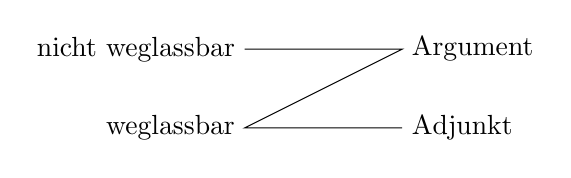
\begin{tikzpicture}

\node[anchor=east](c1) at (-1,2) {nicht weglassbar};
\node[anchor=east](c2) at (-1,1) {weglassbar};
\node[anchor=west](c3) at (1,2) {Argument};
\node[anchor=west](c4) at (1,1) {Adjunkt};
\draw (c1.east) -- (c3.west) -- (c2.east) -- (c4.west);

\end{tikzpicture}

Wenn etwas weglassbar ist, kann es ein Argument oder ein Adjunkt sein.

Wenn es nicht weglassbar ist, ist es ein Argument.

\end{itemize}

}

\frame{
\frametitle{Klausurrelevant}


\includesvg[scale=0.2]{geteilte-Folien/Achtung.svg}

\medskip

Die Definitionen/Eigenschaften für Argumente und Adjunkte sind klausurrelevant. Bitte beachten Sie
die Kontrollfragen und Übungen im Buch.


}